
\documentclass{../download/tPRS2e}

\usepackage{tikz}
\usetikzlibrary{patterns}
\usepackage{graphicx}
\graphicspath{{media/}}

\begin{document}

\title{Some Optimization Models of Tool Path Problem for Sheet Cutting Machines}

\author{
\name{
Petunin A.A.\textsuperscript{a},
Chentsov P.A.\textsuperscript{b}\textsuperscript{a},
Polishuk E.G.\textsuperscript{a},
Ukolov S.S.\textsuperscript{a}$^{\ast}$\thanks{$^\ast$Corresponding author. Email: s.s.ukolov@urfu.ru}
}
\affil{\textsuperscript{a}Ural Federal University, Yekaterinburg, Russia;
\textsuperscript{b}Institute of Mathematics and Mechanics, Ural Branch of the Russian Academy of Sciences, Yekaterinburg, Russia}
}

\maketitle

\begin{abstract}
TODO
\end{abstract}

\begin{keywords}
    thermal cutting;
    discrete optimization;
    toolpath routing;
    technological constraints;
    dynamic programming;
    thermal deformations
\end{keywords}

\section{Introduction}

The problem of cutting tool path optimization
is one of the applied optimization problems arising
in the design of control programs for CNC plate cutting machines.
The cost or time spent is typically used
as objective function to optimize.
The control program is generated by special software 
(Computer-Aided Manufacturing, CAM-system)
just after another well-known optimization problem
has been solved,
i.e. the problem of nesting
(optimal placement of parts to manufacture on the plate).
The task is to minimize the consumption of sheet material
to produce the parts of known shapes, sizes and quantity.
The example of nesting of 24 parts bounded by 30 closed contours
in rectangular area with minimal distance specified is at Fig. \ref{nesting}.
This nesting was obtained by means of Integrated CAD / CAM ``Sirius''.

\begin{figure}[h]
    \begin{center}
    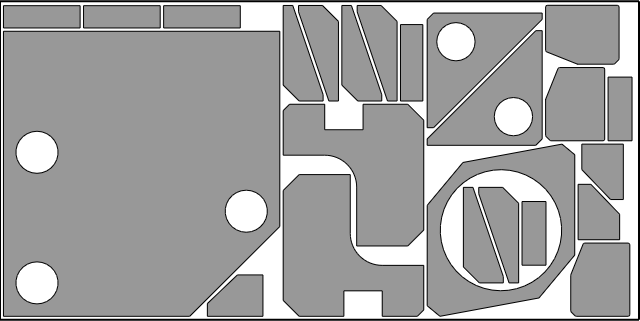
\includegraphics{nesting.png}
    \caption{Example of nesting to a sheet of $2000 \times 1000$ mm
    with minimal distance of $10$ mm} \label{nesting}
    \end{center}
\end{figure}

The process of figure plate cutting with a CNC machine includes
the following activities:
\begin{itemize}
    \item{Pierce point} (cutting start)
    \item{Actual cutting}
    \item{Turning the cutter off} (cutting end)
    \item{Linear movement from end of cut to start of next cut} (air move)
\end{itemize}

Control program usually starts with an air move from
some starting point. Fig. \ref{toolpath} represents
the scheme of cutting two parts with three pierce points.

\begin{figure}[h]
\begin{center}
\tikz{
    \draw[thick,pattern=north east lines, pattern color=gray,even odd rule, rounded corners=2mm]
        (0, 0) ellipse (3 and 2)
        (-2, -1) rectangle (2, 1);
    \draw[thick,pattern=north east lines]
        (7, -1) ellipse (3 and 2);
    \draw[thick]
        (-3, -3) circle(0.05) node[right] {Start of control program};
}
\caption{Example of cutting tool path for two parts and three pierce points} \label{toolpath}
\end{center}    
\end{figure}

The above figure shows tool path going
along the boundary contours of parts,
while in real life it should be offset to
a half cut width in order to preserve parts geometry and sizes.
From the other hand,
most CAM software assume
the path of cutting tool goes
along parts boundaries,
and actual shift is calculated
by CNC machine itself
or special postprocessing software
while converting tool path
from CAM internal representation
to specific CNC machine language.
In the former case,
exact value of cut allowance
is set by CNC machine operator
just before cutting process.
We will further assume
(if not specified otherwise)
that cutting head path is programmed
directly along bounding contours of the parts to cut,
and final tool path contains all the parts contours.
Due to certain technological requirements
pierce points must lay at some extra distance
from part boundaries.
This leads to appearing of additional component,
named ``lead-in''.
In general,
the point of tool switching off
often lay at some
(another) distance from contour to cut,
the resulting tool path addition
is named ``lead-out''
that goes from part boundary to the cut end.
Sometimes lead-out length is allowed to be zero,
causing cutter head to be switched off
directly at the just cut contour.

Let us introduce some notation for tool path components.

We denote $A_1, A_2, \dots A_n$ -- two-dimensional shapes
(closed sets)
that are single- or multiple-connected
regions of Euclidean plane
$\mathbb R^2$.
They are bounded by one or several closed curves
(bounding contours)
$C_1, C_2, \dots C_N,
A_i, C_j \subset \mathbb R^2,
i \in \overline{1, n},
j \in \overline{1, N},
n \leqslant N)$.
Objects $A_1, A_2, \dots A_n$
represent plain parts to cut.

Let also define plane area
$B \subset \mathbb R^2$,
the model of 
sheet material, from which parts are to be cut out.
In general,
this area can be of arbitrary complex shape
(contain several non-rectangular pieces),
but in context of tool path optimization
we will assume it to be
one closed point set bounded
(as well as a detail) by one outer contour.
The holes
(inner contours) are acceptable either.
We will suppose the nesting
(positon of the parts within $B$)
somehow fixed already,
meeting the condition of
mutual non-inersection.
Some other requirements may also arise
due to specific technlogical features
of CNC equipment used.
Any way,
fixed disposition of
$A_1, A_2, \dots A_n \subset B$
is available to us.

Then we denote $S=MM^*$ -- a cutting segment,
i.e. the path of cutting head
from pierce point $M$
to the corresponding cut end point $M^*$.
In terms of geometry,
cutting segment is a curve at Euclidean plane:
$S \subset \mathbb R^2,
M(x,y) \in \mathbb R^2,
M^*(x^*,y^*) \in \mathbb R^2$.
We suppose
the cut direction is defined
in every point of segment $S$.
In case when there are no
closed loops inside segment,
cut direction at each point of segment
is defined uniquely by the starting
point of segment $M$
(pierce point).
Tool path can contain closed loops
not only as part bounding contours,
but also to improve cutting quality.

Using the notion of cutting segment,
all the CNC machine cutting technics
can be classified as:
\begin{enumerate}
    \item{\textit{Closed contour cutting (standard)}}:
    each segment contains exactly one part contour
    that is cut from start to end
    \item{\textit{Multi-segment cutting}}:
    part contour consists of two (or more) cutting segments
    \item{\textit{Multi-contour cutting}}:
    several part contours are cut at once within one cutting segment
\end{enumerate}

\section*{Acknowledgements}

The work was supported by Act 211 Government of the Russian Federation, contract № 02.A03.21.0006

\bibliographystyle{../download/tPRS}
\nocite{*}
\bibliography{en}

\end{document}
